Lorsqu'un langage régulier $L$, représenté par un automate $A_O$ tel que $L(A_O)=L$, est donné à l'oracle d'équivalence, il doit se prononcer sur $L=AL(F)$. Cependant, il ne possède pas d'automate pour $AL(F)$ qui est justement le langage recherché. Il doit alors se prononcer sur l'égalité en se basant uniquement sur $F$.

Comme expliqué dans l'introduction du chapitre, c'est impossible de façon générale. Cependant, en supposant que $AL(F)$ est régulier, il est possible de contourner le problème pour répondre à la question de sécurité.

Contrairement à la version originale de l'algorithme d'Angluin qui a deux possibilités (équivalence ou contre-exemple), celle-ci en a trois. L'oracle peut répondre soit que $AL(F)$ est sécurisé, soit qu'il ne l'est pas, soit que $L$ est différent de $AL(F)$ avec un contre-exemple.


\subsection{$L$ est-il un point fixe de $\mathcal{F}$ ?}

Cette question se base sur le théorème \ref{thm:fl} et en particulier du fait que $AL(F)$ est un point fixe. Il n'est pas possible de prouver que $L=AL(F)$ mais il est possible de montrer que $L\neq AL(F)$ en montrant que $L$ n'est pas un point fixe.

Une façon de montrer que $L\neq AL(F)$, est d'énoncer un seul élément dans $L\bigcup AL(F)-L\bigcap AL(F)=$\alfx l'union exclusive des deux ensembles. Pour rappel, $AL(F)$ est un langage contenant l'ensemble des traces valides pour l'automate à files $F$.

En comparant \fl avec $L$ pour vérifier si $L$ est un point fixe de $\mathcal{F}$, plusieurs situations peuvent apparaître :

\begin{itemize}
  \item $\mathcal{F}(L)-L\neq\emptyset$. Considérons un mot $w\in\mathcal{F}(L)-L$ et montrons que $w\in$\alfx.
  \begin{itemize}
    \item Si $w=t_{q_0}$, c'est que $t_{q_0}\notin L$. Pourtant, par définition, $t_{q_0}\in AL(F)$. Dès lors, $w\in$\alfx
    \item Sinon, si $w$ est une annotation valide, c'est que $L$ n'est pas un point fixe de $\mathcal{F}$. Dès lors, $w$ suffit à démontrer que $AL(F)\neq L$.
    \item Sinon, $w$ n'est pas une annotation valide. $w$ faisant partie de \fl, cela signifie qu'il doit exister un mot $w'\in L$ tel que $w=Post(w')$. Ce $w'$ ne peut pas être une annotation valide : cela impliquerait que $w$ l'est également ce qui est posé comme faux ici. Comme $w'$ n'est pas une annotation valide pour $F$, $w'\notin AL(F)$. Comme $w'\in L$, naturellement $w'\in$\alfx.
  \end{itemize}
  \item $\mathcal{F}(L)\subsetneq L$. Dans ce cas, utilisons la notion de point préfixe. Un ensemble $Z$ est un \emph{point préfixe} d'une fonction $\mathcal{F}$ s'il réduit par son application : $\mathcal{F}$ ($\mathcal{F}(Z)\subseteq Z$). Selon cette définition, $L$ est un point préfixe de $\mathcal{F}$.
  En appliquant $\mathcal{F}$ des deux côtés, ce qui préserve l'inclusion car $\mathcal{F}$ est monotone, on obtient $\mathcal{F}(\mathcal{F}(L))\subsetneq\mathcal{F}(L)$.

  Donc, $\mathcal{F}(L)$ est également un point préfixe. Soit $w\in L-\mathcal{F}(L)$. Comme $w$ n'est pas dans l'intersection de ces deux point préfixes, il ne fait pas partie du point fixe minimum $AL(F)$. En effet, selon la théorie des points fixes de Knaster-Tarski (annexe \ref{app:tarski}), un point fixe minimal est également l'intersection de tous les points préfixes de $\mathcal{F}$.

  \item \fl=$L$. Cela signifie que $L$ est un point fixe de $\mathcal{F}$. Cela signifie qu'il n'est pas possible de prouver que $L\neq AL(F)$ et infirmant cette propriété. Cela ne signifie par pour autant que $L=AL(F)$.

  Ce pourrait très bien être un autre point fixe contenant $AL(F)$ ou un autre ensemble contenant une trace annotée menant à un état qui n'est pas sûr. Pour tenter de continuer à chercher un contre-exemple ou tester la sûreté, il faut poser d'autres questions.

\end{itemize}



\subsection*{$L$ intersecte-t-il avec une région à risque ?}

En visualisant $L$ comme étant un super-ensemble de $AL(F)$ et la région à risque comme un ensemble, il est possible de se représenter les différentes situations envisageables.

\begin{figure}[H]

  \colorlet{circle edge}{black}
  \colorlet{circle area}{blue!20}
  \colorlet{circle darker}{blue!40}
  \tikzset{filled/.style={fill=circle area, draw=circle edge},
    outline/.style={draw=circle edge}}

  \def\circleL{ (0,0) circle (1.5cm) node[right=0.8cm]  {$L$}}
  \def\circleAL{(-0.15,-0.3) circle (1cm) node {$AL(F)$}}

 \centering
 \begin{subfigure}{0.33\textwidth}
  \centering
  \def\circleUS{(0,2.8) circle (1cm) node[text width=1.5cm,align=center]  {Région à risque}}
  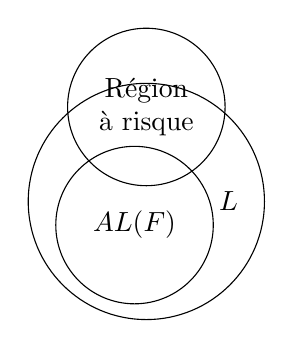
\begin{tikzpicture}
   \draw[outline]\circleL;
   \draw[outline]\circleAL;
   \draw[outline]\circleUS;
  \end{tikzpicture}
  \caption{Pas d'intersection}
 \end{subfigure}%
 \begin{subfigure}{0.33\textwidth}
  \centering
  \def\circleUS{(0,2.2) circle (1cm) node[text width=1.5cm,align=center]  {Région à risque}}
  \vspace{0.6cm}
  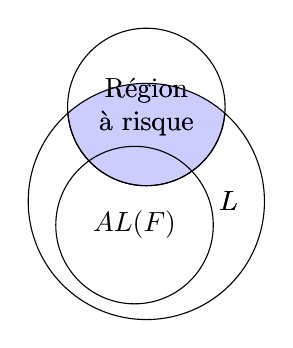
\begin{tikzpicture}
    \begin{scope}
        \clip \circleL;
        \fill[filled] \circleUS;
    \end{scope}
    \draw[outline]\circleL;
    \draw[outline]\circleAL;
    \draw[outline]\circleUS;
  \end{tikzpicture}
  \caption{Intersection avec $L$ seulement}
 \end{subfigure}
 \begin{subfigure}{0.33\textwidth}
   \centering
   \def\circleUS{(0,1.2) circle (1cm) node[text width=1.5cm,align=center]  {Région à risque}}
   \vspace{1.6cm}
   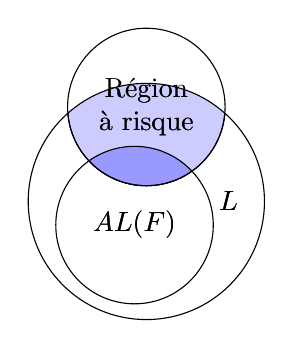
\begin{tikzpicture}
     \begin{scope}
         \clip \circleL;
         \fill[filled] \circleUS;
     \end{scope}
     \begin{scope}
         \clip \circleAL;
         \fill[filled, fill=circle darker] \circleUS;
     \end{scope}
     \draw[outline]\circleL;
     \draw[outline]\circleAL;
     \draw[outline]\circleUS;
   \end{tikzpicture}
  \caption{Intersection avec $AL(F)$}
 \end{subfigure}
 \caption{$L$, $AL(F)$ et la région à risque}\label{fig:inter}
\end{figure}

Pour savoir si nous sommes dans le scénario (a), (b) ou (c) de la figure \ref{fig:inter}, deux tests sont à effectuer.

Premièrement, vérifier si $\mathcal{W}(L)$ est vide ou non. S'il est vide, nous sommes dans le scénario (a) et il est possible d'annoncer avec certitude que $F$ est sécurisé.

\subsection*{Le chemin vers l'état à risque est-il valide ?}

Si la réponse à la question précédente est oui, sommes-nous dans le scénario (b) ou (c) ?
Considérons un des éléments de $\mathcal{W}(L)$. Demandons à l'oracle d'appartenance si ce mot appartient également à $AL(F)$.

Si ce n'est pas le cas, c'est que $L\neq AL(F)$ et que l'algorithme d'Angluin peut continuer grâce au contre-exemple fourni. Ici, il peut s'agir soit d'un scénario (b) soit d'un scénario (c) puisqu'un autre mot de $\mathcal{W}(L)$ pourrait appartenir à $AL(F)$. Cela correspondrait à prendre un mot de la zone bleue claire dans (c).

Améliorer l'approximation d'$AL(F)$ permet justement de mieux discriminer ces deux scénarios sans devoir consulter la totalité de $\mathcal{W}(L)$.

Si par contre le mot étudié appartient aussi à $AL(F)$, on a un mot étant à la fois dans $AL(F)$ et dans la région à risque. $F$ est déclaré à risque et le mot est retourné comme contre-exemple. Il s'agit du scénario (c).
